% !Mode\dots ``TeX:UTF-8''
% !TEX root = ../bare_jrnl.tex

\section{Algorithm for online observability}
\label{sec:deter}
To  determine  online observability of \BCN s, one needs to determine $\Ks(\Ded(\Delta_N,\varepsilon,\mathsf{o}^{j}(0)))$ for every non-empty $\Ded(\Delta_N,\varepsilon, \mathsf{o}^{j}(0))$. 

\subsection{Input-labelled graph}
We start with input-labelled graph $\mathcal{G}=(\mathcal{V}, \mathcal{E}, \mathcal{L})$.

\begin{definition}[Input-labelled Graph]
Let $\mathcal{V}$, $\mathcal{E}$ and $\mathcal{L}$ be the vertex set, the edge set and the labelling function of an input-labelled graph $\mathcal{G}=(\mathcal{V}, \mathcal{E}, \mathcal{L})$. $\mathcal{G}$ is called the input-labelled graph of the \BCN\, if 
\begin{itemize}
\item  $\mathcal{V}=\{\mathsf{S}\in\bigcup_{j=0}^{(2^m -1)} 2^{\Ded(\Delta_N,\varepsilon,\delta^j_{2^m} )}|\ \Ks(\mathsf{S})\ne \infty\}$;
\item  $\mathcal{E}=\{(\mathsf{S}_1,\mathsf{S}_2)\in \mathcal{V}\times \mathcal{V}|$ there is an $\mathsf{i} \in \Delta_M$ such that $|\Ded\left(\mathsf{S}_1,\mathsf{i},\varepsilon\right)|=|\mathsf{S}_1|$, and for every $\Ded(\mathsf{S}_1,\mathsf{i},\mathsf{o}^{j})\neq \emptyset$ $\Ded(\mathsf{S}_1,\mathsf{i},\mathsf{o}^{j})\in \mathcal{V}$, $\mathsf{S}_2\in\{\Ded(\mathsf{S}_1,\mathsf{i},\mathsf{o})| \Ded(\mathsf{S}_1,\mathsf{i},\mathsf{o})\neq \emptyset, \mathsf{o}\in \Delta_Q\}\}$;
\item  $\mathcal{L}:\mathcal{E}\mapsto 2^{\Delta_M}=(\mathsf{S}_1,\mathsf{S}_2)\mapsto\{\mathsf{i}\in \Delta_M|$ $|\Ded\left(\mathsf{S}_1,\mathsf{i},\varepsilon\right)|=|\mathsf{S}_1|$, and for every $\Ded(\mathsf{S}_1,\mathsf{i},\mathsf{o}^{j})\neq \emptyset$, $\Ded(\mathsf{S}_1,\mathsf{i},\mathsf{o}^{j})\in \mathcal{V}$, $\mathsf{S}_2\in\{\Ded(\mathsf{S}_1,\mathsf{i},\mathsf{o})| \Ded(\mathsf{S}_1,\mathsf{i},\mathsf{o})\neq \emptyset, \mathsf{o}\in \Delta_Q\}\}$.
 \end{itemize}
\end{definition}

\begin{figure}[thpb]
      \centering
      \framebox{\parbox{3in}{
		\centerline{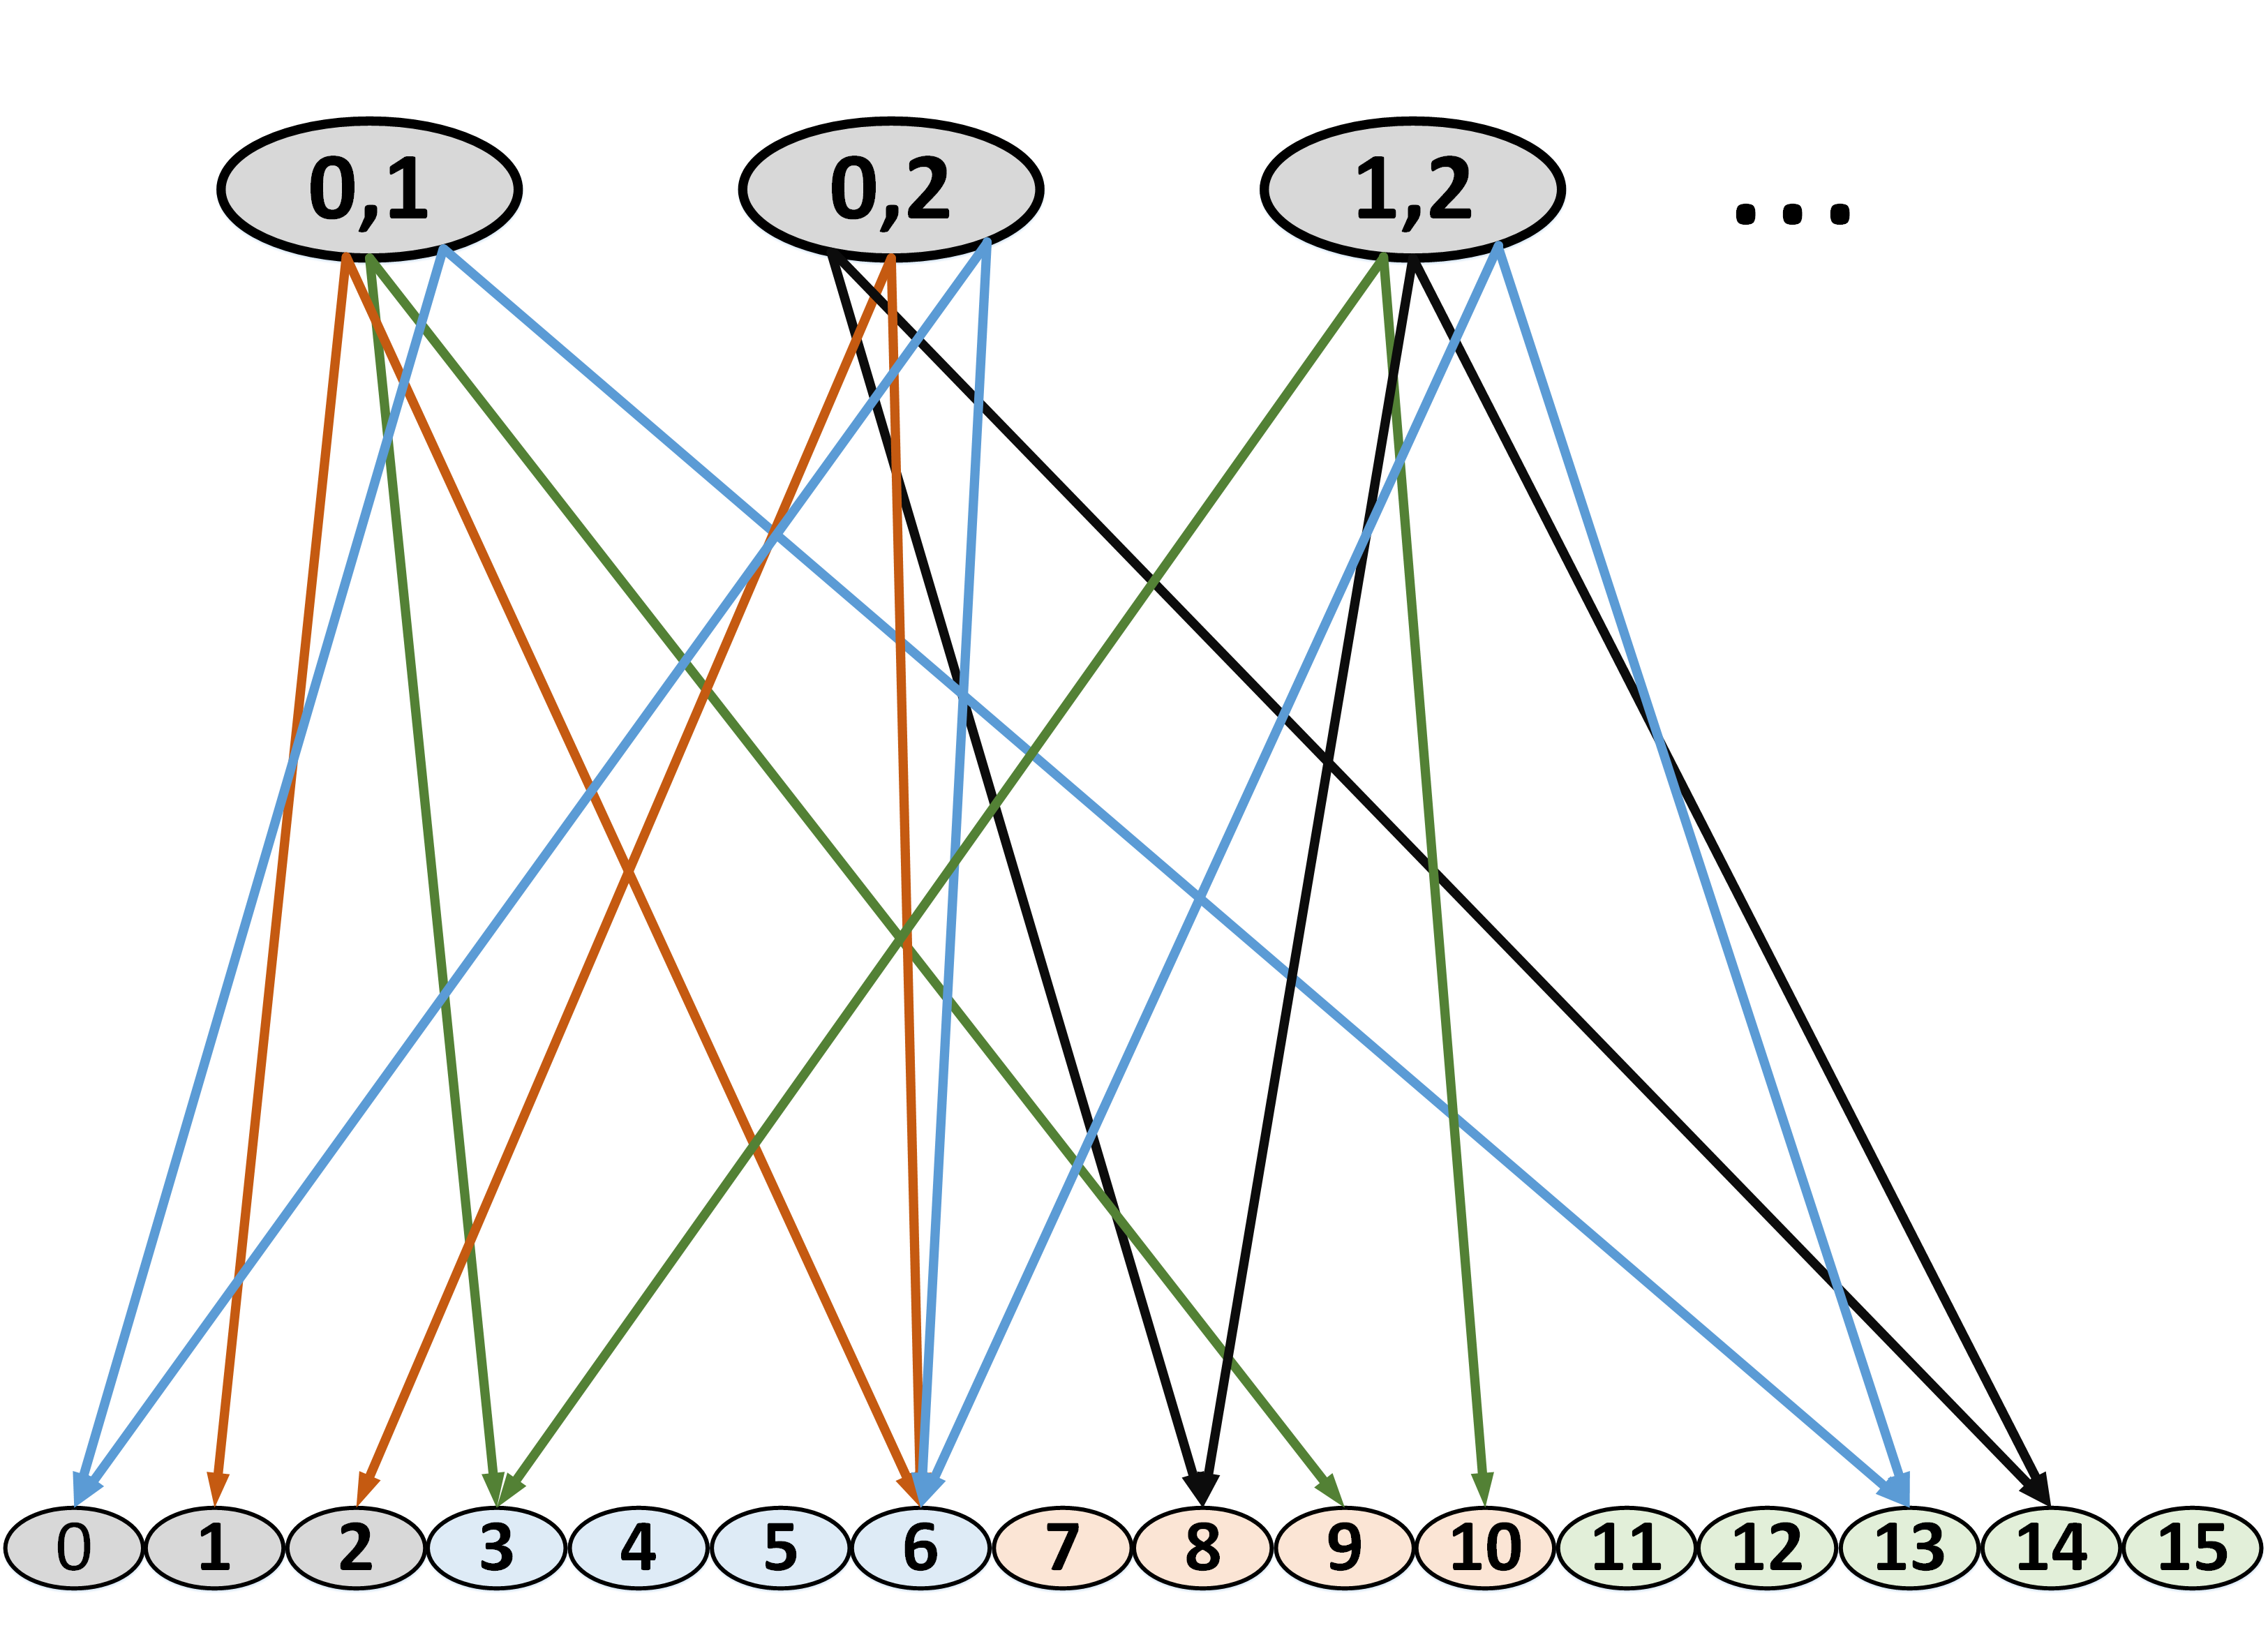
\includegraphics[scale=0.090]{figures/Fig4.png}}
	}}
      \caption{Part of the input-labelled graph, where the green, black, orange, blue edges are labelled with $\{\delta_4^0\}$, $\{\delta_4^1\}$, $\{\delta_4^2\}$ and $\{\delta_4^3\}$ respectively.}
      \label{fig:4}
\end{figure}

Intuitively, $\mathcal{V}$ represents all of the state sets $\mathsf{S}$ which satisfy $\Ks(\mathsf{S})\ne \infty$ and every $\mathsf{s}^i\in\mathsf{S}$ with identical corresponding output, $\mathcal{E}$ represents the relation between $\mathcal{V}$, and $\mathcal{L}$ label every $\mathsf{e}^j \in\mathcal{E}$ with a set of inputs based on the definition of $\Ks(\mathsf{S})$. %Thus we can determine $\Ks(\Ded(\Delta_N,\varepsilon,\mathsf{o}^{j}(0)))$ of every non-empty $\Ded(\Delta_N,\varepsilon, \mathsf{o}^{j}(0))$ by checking the input-labelled graph.

%From the {\em Lemma \ref{lemm:1}}, we have that if for the set of states $\mathsf{S}^1$ there does not exist any $k^{1}\ge 0$ such that $\mathsf{S}^{1}$ is $k^{1}$-step determinable, and $\mathsf{S}^{1}\subseteq \mathsf{S}^{2}$. Then there does not exist any $k^{2}\ge 0$ that make $\mathsf{S}^{2}$ $k^{2}$-step determinable. Therefore, i

In the process of building input-labelled graph for a \BCN, we build the vertexes with fewer states at first, and then build the vertexes with more states.
\begin{itemize}
\item  Firstly, once we find a $\mathsf{S}^i$ that $\Ks(\mathsf{S}^i)= \infty$, and there exists $\mathsf{o}^{j}\in \Delta_Q$ that $\mathsf{S}^{i}\subseteq \Ded(\Delta_N,\varepsilon, \mathsf{o}^{j})$, we have $\Ks(\Ded(\Delta_N,\varepsilon, \mathsf{o}^{j}))= \infty$ based on the {\em Lemma \ref{lemm:1}}, then the \BCN\ is not online observable.
\item  Secondly, from the {\em Lemma \ref{lemm:2}}, as we have determined $\Ri(\mathsf{S}')$ for every $\mathsf{S}'\subset\mathsf{S}$, we can preliminarily determine $\Ri(\mathsf{S})$.
 \end{itemize}
 \subsection{Determination algorithm}
 Then we propose the {\bf Algorithm~\ref{alg:1}} to determine online observability based on input-labelled graph.%, and it can find all paths to determine $\mathsf{s}(0)$ if the \BCN\ is online observable.

\begin{description}
\item[Step 1]  For every $n>0$ we try to build vertexes with $n$ states which with identical corresponding output. 
\item[Step 2] If the vertexes can  be built, when $n>1$, we check the $\Ks(\mathsf{S}^i)$ of every vertex and build edges for it. If there is a vertex without any edge, then the \BCN\ is not online observable.
\item[Step 3] Else if we can not build any vertex with $n$ states, then  for every non-empty $\Ded(\Delta_N,\varepsilon, \mathsf{o}^{j}(0))$, $\Ks(\Ded(\Delta_N,\varepsilon, \mathsf{o}^{j}(0)))\ne\infty$, the \BCN\ is online observable.
 \end{description}

\begin{algorithm}[h]
\caption{Determination algorithm}
\begin{algorithmic}[1]
\REQUIRE 
The updating rules of \BCN
\ENSURE  
The input-labelled graph of \BCN
\STATE Boolean value $Ob=$ true 
\STATE integer $i$ , $j$, $n=1$\
\STATE array $VertexArray[\ ]$, $InputArray[\ ]$
\STATE {\sf buildvertex}($n$)
\STATE $VertexArray=${\sf buildvertex}($++n$)
\WHILE {($VertexArray!=$Null)}
\FOR{($i=0$; $i<arraysize(VertexArray)$; $i++$)}
\IF{($p==2$)}
\STATE $InputArray$ = $\Delta_M$ 
\ELSE

\STATE Find $InputArray$ by other vertexes

\ENDIF
\FOR{($j=0$; $j<arraysize(InputArray)$; $j++$)}
\STATE Check $VertexArray[i]$ by $InputArray[j]$ 
\STATE Build edges for $VertexArray[i]$ 
\ENDFOR
\IF {($VertexArray[i]$ has not any edge)}
\STATE  $Ob=$ false 
\STATE return Null
\ENDIF
\ENDFOR
\STATE $VertexArray=${\sf buildvertex}($++n$)
\ENDWHILE
\STATE return $\Delta_N$\
\end{algorithmic}
 \label{alg:1}
\end{algorithm}
\begin{algorithm}[h!]
\caption{{\sf buildvertex}(integer $n$)}
\begin{algorithmic}[1]
\REQUIRE 
The number of states $n$
\ENSURE  
The vertexes with $n$ states which with identical corresponding outputs 
\STATE  Build all vertexes with $n$ states 
\IF{(Failed to build)} 
\STATE  return Null
\ELSE 
\STATE  Classify these vertexes
\STATE Sort the states in these vertexes
\STATE Sort these vertexes
\STATE return vertexes
\ENDIF 
\end{algorithmic}
 \label{alg:2}
\end{algorithm}

Some details of {\bf Algorithm~\ref{alg:1}} and {\bf Algorithm~\ref{alg:2}}:
\begin{itemize}
\item Build all vertexes with $n$ states:
\begin{description}
\item[Step 1] For every non-empty $\Ded(\Delta_N,\varepsilon,\mathsf{o}^{j})$, if $n>|\Ded(\Delta_N,\varepsilon,\mathsf{o}^{j})|$, then we could not get any set with $n$ states from $\Ded(\Delta_N,\varepsilon,\mathsf{o}^{j})$. Else we can get $\frac{(|\Ded(\Delta_N,\varepsilon,o_j)|)!}{n!\times (|\Ded(\Delta_N,\varepsilon,o_j)|-n)!}$ sets of states from $\Ded(\Delta_N,\varepsilon,\mathsf{o}^{j})$, where $n!$ is the factorial of $n$.
\item[Step 2] Using all of the sets of states got in Step 1 to build vertexes. 
\end{description}
 \item Sort the states in these vertexes and sort these vertexes: We sort the states inside the vertexes at first, and then sort the vertexes by the states of them. For example, in Fig.~\ref{fig:4} the vertexes $\{\delta_{16}^0,\delta_{16}^1\}$, $\{\delta_{16}^0,\delta_{16}^2\}$ and $\{\delta_{16}^1,\delta_{16}^2\}$ are well shorted. 
  \item Find $InputArray$ by other vertexes:
   For the vertex $VertexArray[i]$ contains $n$ sorted states, we use the vertexes with the first $(n-1)$ states and the last $(n-1)$ states to find $InputArray$ for $VertexArray[i]$. For example, in Fig.~\ref{fig:4}, $\Ri(\{\delta_{16}^0,\delta_{16}^1\})=\{\delta_{4}^0,\delta_{4}^2,\delta_{4}^3\}$ and $\Ri(\{\delta_{16}^1,\delta_{16}^2\})=\{\delta_{4}^0,\delta_{4}^1,\delta_{4}^3\}$. We take the intersection of them to be $InputArray$ of $\{\delta_{16}^0,\delta_{16}^1,\delta_{16}^2\}$ i.e. $InputArray=\{\delta_{4}^0,\delta_{4}^3\}$. 
  \item Check $VertexArray[i]$ by $InputArray[j]$:
     
\begin{itemize}
\item If the $|\Ded(VertexArray[i],InputArray[j],\varepsilon)|<|VertexArray[i]|$, then the $InputArray[j]$ is a wrong input.
\item Else if every non-empty \\$\Ded\left(VertexArray[i],InputArray[j],\mathsf{o}^{p}\right)$ already exists in the directed graph, then connect $VertexArray[i]$ to it and labell the edge with $InputArray[j]$, else we check it latter. 
\end{itemize} 
\end{itemize} 


%With the algorithm based on directed graph we can find all paths to determine the initial state of a \BCN. Thus, at time step $t$, we can use the $\mathsf{S}(t)$ and the directed graph to derive all of the input $\mathsf{i}(t)$ which can help us determine $\mathsf{s}(0)$. While, there comes a problem. Which input is the best input? To solve this problem, in the {\em Section \ref{sec:app}}, we will present how to decide the input to get better performance.
